\begin{pastexam}[label={px:ntu-108-comm-dsab-19}]{臺大電信所 108 學年度（B）第 19 題}
（單選；每題 2.5 分，答錯不倒扣）

Consider the AVL tree in Figure 1. After inserting key 60, what's the parent of the node with key 87?

A.~42 \qquad B.~60 \qquad C.~66 \qquad D.~73 \qquad E.~94

\begin{center}
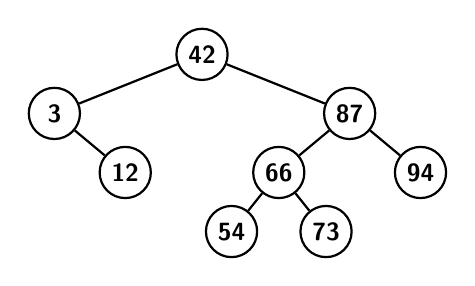
\begin{tikzpicture}[x=0.75cm,y=0.75cm,v/.style={circle,draw,thick,inner sep=0pt,minimum size=6.5mm,font=\sffamily\bfseries\small}]
\node[v] (n42) at (2.5,0) {42};
\node[v] (n3) at (0,-1) {3};
\node[v] (n87) at (5,-1) {87};
\node[v] (n12) at (1.2,-2) {12};
\node[v] (n66) at (3.8,-2) {66};
\node[v] (n94) at (6.2,-2) {94};
\node[v] (n54) at (3,-3) {54};
\node[v] (n73) at (4.6,-3) {73};
\draw[thick] (n42) -- (n3); \draw[thick] (n42) -- (n87); \draw[thick] (n3) -- (n12);
\draw[thick] (n87) -- (n66); \draw[thick] (n87) -- (n94);
\draw[thick] (n66) -- (n54); \draw[thick] (n66) -- (n73);
\end{tikzpicture}\\
Figure 1: AVL Tree
\end{center}
\end{pastexam}

\begin{pastsoln}
答案是 C。

先算原樹每個節點的高度（葉節點高度 $0$）：$54, 73, 94, 12$ 是 $0$；$66$ 是 $1$；$3$ 是 $1$；
$87$ 是 $2$；$42$ 是 $3$。 每個節點左右高度差都不超過 $1$，是合法的 AVL 樹。

插入 $60$：$60 > 42$ 往右，$60 < 87$ 往左，$60 < 66$ 往左，$60 > 54$，成為 $54$ 的右子節點。
從 $60$ 往上更新高度、檢查平衡因子（左高減右高，資結書第~10.2.3~節）：
\begin{itemize}
\item $54$：左 $-1$（空）、右 $0$，高度 $1$，平衡因子 $-1$，沒事。
\item $66$：左 $1$、右 $0$（$73$），高度 $2$，平衡因子 $+1$，沒事。
\item $87$：左 $2$（$66$）、右 $0$（$94$），平衡因子 $+2$，\textbf{失衡}。
\end{itemize}
新節點在 $87$ 的左子節點 $66$ 的\textbf{左}子樹裡（$60$ 在 $54$ 底下），是 LL 型，在 $87$ 做一次
右旋：$66$ 升上來取代 $87$ 的位置，$87$ 變成 $66$ 的右子節點，$66$ 原本的右子樹 $73$ 改掛成
$87$ 的左子節點。
\begin{center}
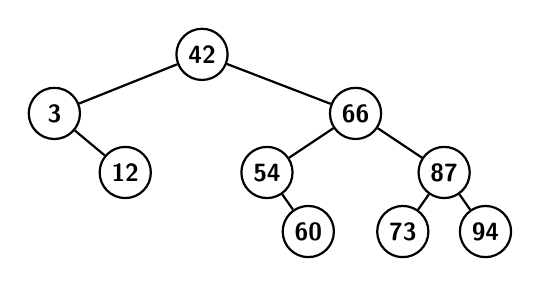
\begin{tikzpicture}[x=0.75cm,y=0.75cm,v/.style={circle,draw,thick,inner sep=0pt,minimum size=6.5mm,font=\sffamily\bfseries\small}]
\node[v] (n42) at (2.5,0) {42};
\node[v] (n3) at (0,-1) {3};
\node[v] (n66) at (5.1,-1) {66};
\node[v] (n12) at (1.2,-2) {12};
\node[v] (n54) at (3.6,-2) {54};
\node[v] (n87) at (6.6,-2) {87};
\node[v] (n60) at (4.3,-3) {60};
\node[v] (n73) at (5.9,-3) {73};
\node[v] (n94) at (7.3,-3) {94};
\draw[thick] (n42) -- (n3); \draw[thick] (n42) -- (n66); \draw[thick] (n3) -- (n12);
\draw[thick] (n66) -- (n54); \draw[thick] (n66) -- (n87); \draw[thick] (n54) -- (n60);
\draw[thick] (n87) -- (n73); \draw[thick] (n87) -- (n94);
\end{tikzpicture}
\end{center}
旋轉後子樹的高度回到 $2$，和插入前一樣，$42$ 不用再調整（左 $1$、右 $2$）。 $87$ 的父節點是
$66$，選 C。 A 的 $42$ 是旋轉前的祖父；D 的 $73$ 現在是 $87$ 的左子節點，不是父節點。
\end{pastsoln}
